\documentclass[tikz]{standalone}
\usepackage{tikz}
\usetikzlibrary{calc,positioning, shapes, petri, automata}
\tikzset{
    transV/.style={transition, fill=black, minimum height = 12mm, minimum width = 1.5mm,inner sep = 0mm},
    transH/.style={transition, fill=black, minimum width = 12mm, minimum height = 1.5mm,inner sep = 0mm},
    node distance=1.5
}
\usepackage{amsmath,amssymb,amsthm,mathrsfs,amsfonts}

\usepackage{csquotes}
\usepackage{booktabs}

\usepackage{graphicx}
\graphicspath{ {../img/} }

\newcommand{\LSset}[2]{\scriptsize $\begin{aligned}&\{#1\}_L\\&\{#2\}_S\end{aligned}$}


\begin{document}    
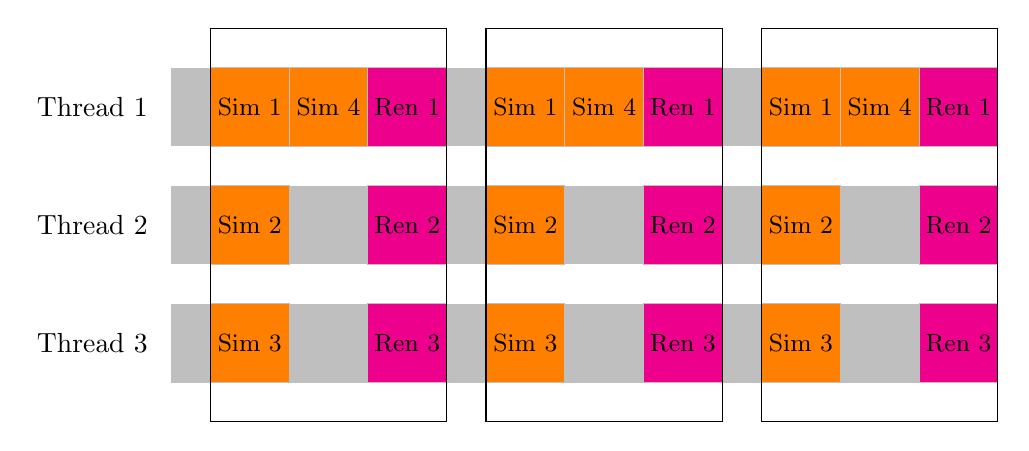
\begin{tikzpicture}
	\fill[lightgray]  (0,0) rectangle (10,1);
	\fill[lightgray] (0,-1.5) rectangle (10,-0.5);
	\fill[lightgray]  (0,1.5) rectangle (10,2.5);
	
	\node at (-1,2) {Thread 1};
	\node at (-1,0.5) {Thread 2};
	\node at (-1,-1) {Thread 3};

	\foreach \i in {0,3.5,7}{
	\fill [orange,draw=lightgray] ($(\i,0) + (0.5, 1.5)$) rectangle ($(\i,0) +(1.5, 2.5)$);
	\fill [orange,draw=lightgray] ($(\i,0) + (0.5,-1.5)$) rectangle ($(\i,0) +(1.5,-0.5)$);
	\fill [orange,draw=lightgray] ($(\i,0) + (1.5, 1.5)$) rectangle ($(\i,0) +(2.5, 2.5)$);
	\fill [orange,draw=lightgray] ($(\i,0) + (0.5, 0.0)$) rectangle ($(\i,0) +(1.5, 1.0)$);
	
	\fill [magenta,draw=lightgray] ($(\i,0) + (2.5, 1.5)$) rectangle ($(\i,0) + (3.5, 2.5)$);
	\fill [magenta,draw=lightgray] ($(\i,0) + (2.5, 0.0)$) rectangle ($(\i,0) + (3.5, 1.0)$);
	\fill [magenta,draw=lightgray] ($(\i,0) + (2.5,-1.5)$) rectangle ($(\i,0) + (3.5,-0.5)$);
	
	\draw  ($(\i,0) + (0.5,3)$) rectangle ($(\i,0) + (3.5,-2)$);
	
	\node[font=\small] at ($(\i,0) + (1,2)$) {Sim 1};
	\node[font=\small] at ($(\i,0) + (1,0.5)$) {Sim 2};
	\node[font=\small] at ($(\i,0) + (1,-1)$) {Sim 3};
	\node[font=\small] at ($(\i,0) + (2,2)$) {Sim 4};
	\node[font=\small] at ($(\i,0) + (3,2)$) {Ren 1};
	\node[font=\small] at ($(\i,0) + (3,0.5)$) {Ren 2};
	\node[font=\small] at ($(\i,0) + (3,-1)$) {Ren 3};

	}
	\end{tikzpicture}
\end{document}